\chapter{Introduction}

%Replace \lipsum with text.
% You may have as many sections as you please. This is just for reference.

\section{Objective}
The objective of  this project is to achieve decentralization in governance through the mobile applications. It aims in the delegation of power in the hands of local community people known as human access points (HAPs) to foster local governance. Panchayat members will be given an Android phone pre-loaded with a local governance application which is used for the dissemination of information to the local community people. These volunteers will use installed mobile application for the broadcasting of audio announcements, sending of quick text messages to the registered members of the community. Application will also be used to launch the recent ongoing surveys to the relevant target members of the community. It will help in community monitoring, improving awareness, spreading of social welfare information, dispersing information related to government schemes and other livelihood services.

\section{Motivation}
We can see various regions of India where information unreachability is a major concern. In the modern era, smart phones have  become a massive infotainment tool which can be used for the information reachability in resource lagging areas. Also, E-government and related Information and Communication Technology (ICT) are commonly understood to provide a great opportunity to innovate the business of government by fostering efficiency and reforming public management \cite{ict1}.

Firstly, People of rural areas are deprived of these smart phones which is the key reason of information deprivation among these people. Secondly, administrative people working top in the hierarchy are unaware of the local community problems. Thirdly, rural people are poorly literate which hinders them from the information. 

Keeping above problems in mind, delivering of voice messages on the basic phones of the local people by their own community members using mobile applications is the best tool for information dissemination. Local people (panchayat members/ HAPs/ Volunteers) can serve their community better.  Voice messages become accessible to even poorly literate people. Also, Voice calls will help poor people in a better way. With a mobile service subscriber base of  377.73 million in rural areas as on March 2014, it indeed is a good idea to use mobile to bring local governance among the community people and foster social change \cite{ruralbase:online}. Delegating information through mobile phones to such a  large subscriber mobile base will effectively help in managing local issues of the local people by the volunteers.

\section{Brief Description}
Decentralization is the process of redistributing or dispersing functions, powers, people or things away from a central location or authority \cite{bardhan2002decentralization}. Decentralization provides the opportunity for a wider diversity of innovations, and increases flexibility of government in the context of changing circumstances. This is so because the decentralized, participatory model of governance mainstreams the many groups of citizens that were previously excluded, and creates greater scope for local and community self management. This means that the vast reservoir of talent, innovativeness, creativity, problem solving capacity and leadership qualities which have previously laid dormant in the local population is now able to find expression, and can be applied to the problems, visions and aspirations of the local community, and will also be available to contribute to nation building. \cite{Decentral:online}.

\subsection{Advantages of Decentralization}

\begin{enumerate}

\item \textbf{Better control and supervision} \\
Decentralisation ensures better control and supervision as the subordinates at the lowest levels will have the authority to make independent decisions. As a result they have thorough knowledge of every assignment under their control and are in a position to make amendments and take corrective action.

\item \textbf{Quick Decision-Making} \\
Decentralisation brings decision making process closer to the scene of action. This leads to quicker decision-making of lower level since decisions do not have to be referred up through the hierarchy.

\item \textbf{Facilitates diversification}\\
Under decentralization, the diversification of products, activites and markets etc., is facilitated. A centralised enterprise with the concentration of authority at the top will find it difficult and complex to diversify its activities and start the additional lines of manufacture or distribution.

\item \textbf{Executive Development}\\
When the authority is decentralised, executives in the organisation will get the opportunity to develop their talents by taking initiative which will also make them ready for managerial positions. The growth of the company greatly depends on the talented executives.

\item \textbf{It promotes motivation}\\
To quote Louis A. Allen, “Decentralisation stimulates the formation of small cohesive groups. Since local managers are given a large degree of authority and local autonomy, they tend to weld their people into closely knit integrated groups.” This improves the morale of employees as they get involved in decision-making process.

\end{enumerate}

\begin{figure}[H]
    \centering
	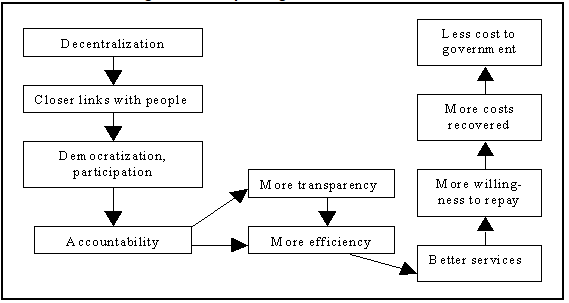
\includegraphics[width=0.8\textwidth]{Decentral.png}
    \caption{ Advantages of Decentralization of Governance }
    \label{fig:Advantages of Decentralization of Governance}
\end{figure}

% [image source - http://www.fao.org/docrep/005/y2006e/y2006e05.gif]

Consequently, the designed application will be used by the volunteers for the easy dispersal of information to the local people. People will remain informed about the ongoing government schemes, daily livelihood services and other local news. Participation in the ongoing surveys will also be managed and tracked easily. Delegation of community monitoring in the hands of volunteers will help in achieving the decentralization of governance effectively. 

\section{Literature Review and Related Work}
India is witnessing a phenomenal increase in mobile phone usage particularly in rural India over the last few years. Mobile handsets have become affordable and feature-rich making them amenable to value added applications. There is a consensus among mobile service providers, mobile content developers, banks and other financial institutions, policy makers (i.e., Reserve Bank of India, Ministry of Panchayat and Rural development), and various regulators (i.e., Telecom Regulatory authority of India, Indian Banks association, Insurance regulator of India, Mobile service provider association) that mobile applications is a viable way to reach information and service to rural people. The following papers were reviewed while developing the concept.

\begin{itemize}

\item Emergent Practices Around CGNet Swara, A Voice Forum for Citizen Journalism
in Rural India, ICTD’12 \cite{cgnet} : This paper talks about the initiative of CGNet Swara,
which is a project similar to JMR active in Chhatisgarh. The authors explain the
deployment of the system, and their experiences. It also delves into qualitative
and quantitative analysis of the data coming in, of the callers, topic about which
stories were reported among other things.

\item Designing Mobile Interfaces for Novice and Low-Literacy Users,ACM Transactions
on Computer-Human Interaction. 2011 \cite{design}: This study explores different interfaces
for low-literacy and novice mobile users. The authors conducted two studies com-
paring text-based interfaces to other different alternatives such as, one: automatic
solutions including graphics, spoken dialog and text-free user interfaces and sec-
ond: a live human operator. Based on these studies and interviews conducted
with the subjects, the authors cite results regarding the comfort of novice users
with the different mobile interface components. They also lay down certain design
recommendations while designing mobile user interfaces for such users.

\item Citizen Connect SMS Mobile Application \cite{Decen5:online} : This mobile application empowers citizens with access to information and grievance redressal of local government services.SMC was launched to provide latest information and facts to people and take the government services to the doorsteps of the citizens. They launched a mobile app ‘Citizens Connect’ that enables information sharing and service providing through latest technology.  The mobile app, which can be downloaded free of cost on Android phones, provides information regarding elected and administrative wings, registration procedures, recruitment advertisements and even rainfall. Users can also check birth and death certificate details, property tax details, pay water meter bills and share feedback. Having launched in 2013, the app has already received over 18 million service requests and 7400 complaints.


\item Mygaon, Web Platform \cite{MyGao25:online} : The initiative is centered around India’s 6.4 lakh villages, and more importantly, their efforts towards ensuring that each of native village is prosperous, healthy, and safe place to live. Mygaon's vision is to create a comprehensive, dynamic and interactive web platform of information on villages in India in order to facilitate impactful and accelerated social change.On My Gaon, one is able to browse through real-time information on villages in India in a rich and visual manner. One can also view information regarding verified organizations which are involved in successful and highly impactful projects in these locations. They introduce 'Village Champions' - individuals on the ground who are willing to help community people make a lasting impact in the villages and thus provide them with all the information, tools and networks one need to contribute to one's native village.

\item Rural ICT : Rural Information and Communication Technology (ICT) is a software platform that leverages cheap mobile phones and opportunistic Internet access for commercial purposes as well as group-based knowledge exchange. Users interact with the platform by dialing a phone number and navigating simple automated prompts using touchtone keys. It is a knowledge sharing system built for telephony, which empowers its users to engage in conversation, trade or exchange of ideas in any language and with any community, thus surmounting literacy and language challenges. The voice portal is a 24-hr system where customers can record their order any time, it will thus help in saving time, effort and money. Orders placed would be easily manageable, can be tracked and avoid any loss or missing orders. There is no limitation on no. of user availing this facility in a group and thus also can be used for public surveying. This automating of job is to set an online system - to process transactions and announcements.

There are three users of the system named as admins, publishers and the members. The customers register to the system as members. The publisher along with the permission of the admin will handle the system and broadcast messages to respective customers.The members of the system, the customers can place their request on the system. It may be in the form of an order, a feedback or a response. All their response and request will be stored in the system and the publisher or the admin will make sure that the order is being processed successfully. Thus with the help this system, one can record a message (special offers or notifications) to be broadcasted.

\item Comparing Semiliterate and Illiterate Users Ability to Transition from Audio+Text
to Text-Only Interaction, CHI’09 \cite{findlater2009comparing} : In this paper, the authors establish fact that
illiterate and semi-literate users can’t be both clubbed together into one category
when it comes to designing suitable user interfaces for them. This is so because for
users with some basic literacy, who though might not be able to read and write flu-
ently, text provides an unambiguous mode of interaction. The authors conducted
studies where they found that when semi-literate users were presented with an
interface with both text and audio support, they soon reduced their dependence
on audio while no such improvement was found in case of the fully illiterate users.
The paper provides interesting insights into the differences in the responses of fully
illiterate and semi-literate users to different UI components.
\end{itemize}
% You may add figures in the following manner.

